\chapter{Sekcja Elektroniczna}
Projekt elektroniczny na potrzeby tej pracy został ograniczony do minimum i był częściowo wzorowany na sekcji elektronicznej projektu Zebulon 2.0. Zasilanie składa się z akumulatora typu LiPo i minimum dwóch przetwornic. Jako mózg urządzenia zastosowany został minikomputer Raspberry Pi 4B i to do jego zasilenia potrzebna jest jedna z przetwornic. Zgodnie z dokumentacją Raspberry zasilanie jest ze źródła o napięciu $5V$ i prądzie przynajmniej $3A$.\cite{RPI_power_sup} Dlatego została wybrana przetwornica D36V28F5 (Pololu 3782). Natomiast ze względu na brak dostępności zakupiono i  zainstalowano przetwornicę D36V50F5 (Pololu 4091) (Rys. \ref{img:voltage_converters}, po lewej), która to niewiele różni się ceną, ale za to ma lepszy prąd wyjściowy. \cite{polulu_step_down}\\

\begin{figure}[h!]
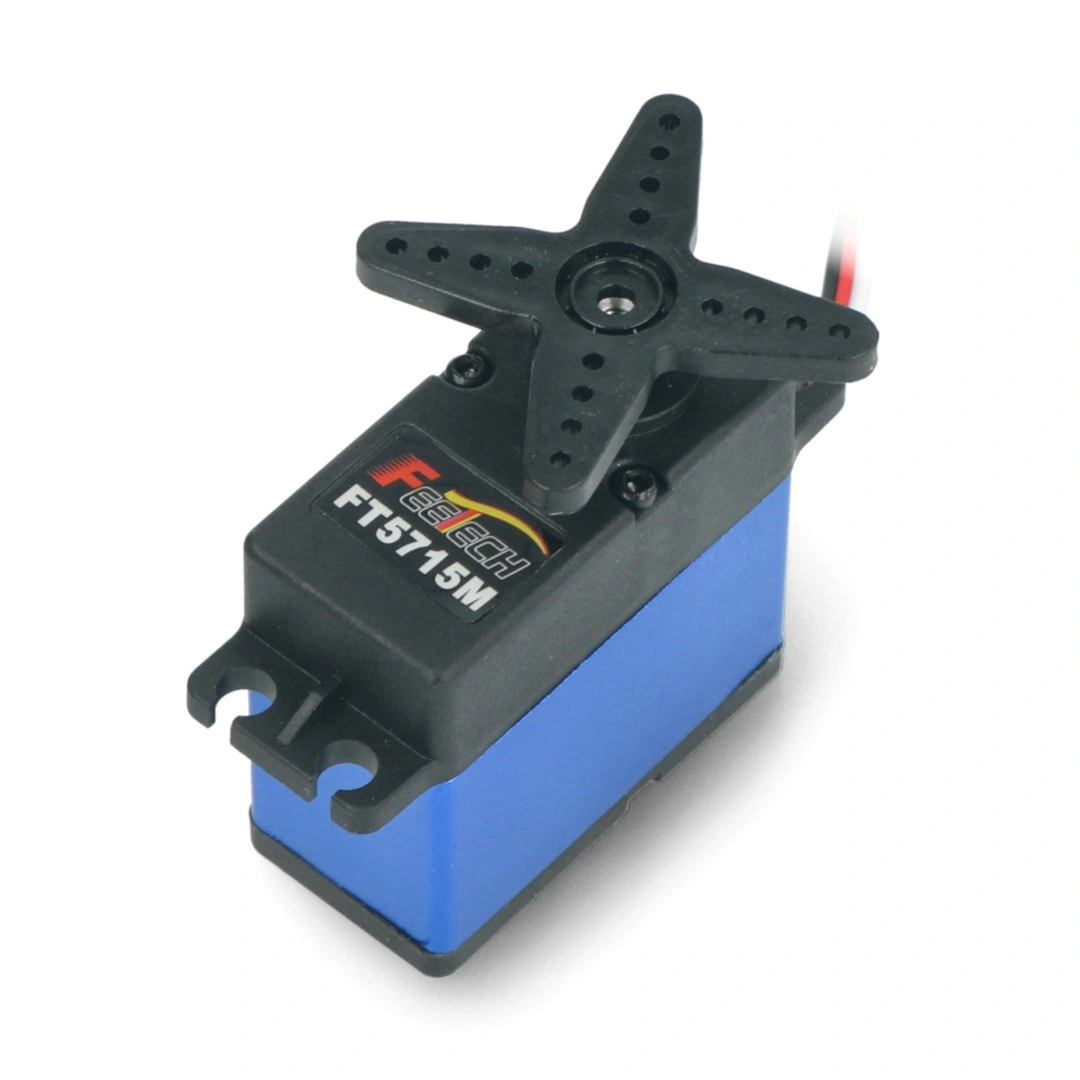
\includegraphics[width=0.5\textwidth]{img/feetech.png}
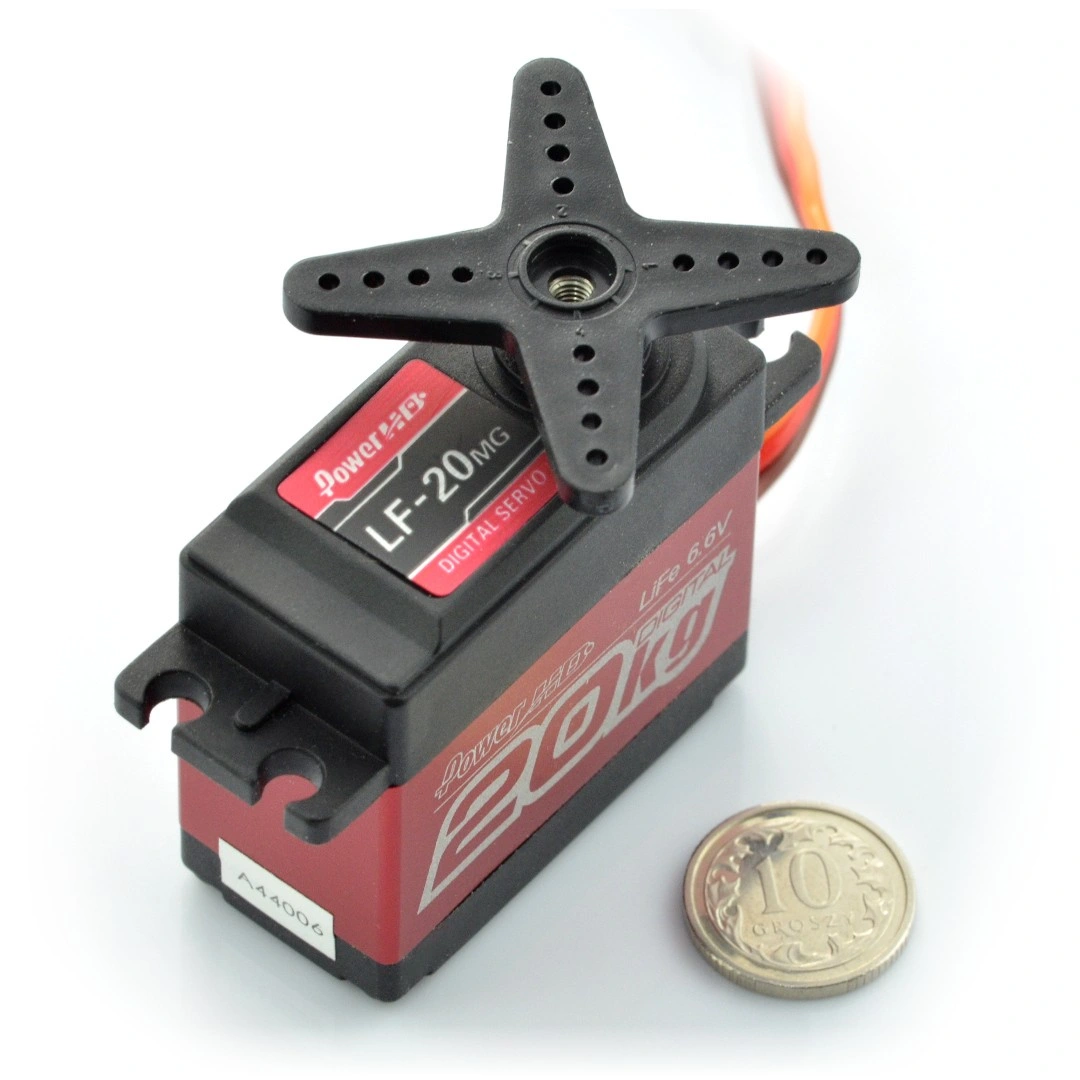
\includegraphics[width=0.5\textwidth]{img/powerhd.png}
\caption{Serwomechanizmy wybrane do projektu. \cite{feetech_docs} \cite{powerhd_docs}}
\label{img:servos}
\end{figure}

Druga przetwornica ma za zadanie zasilić serwomechanizmy. Serwomechanizmy wybrane do tego projektu to Feetech FT5715M (sztuk 3) i PowerHD LF-20MG (sztuk 6). (Rys. \ref{img:servos}) W czasie zakupu serwa te wypadały najlepiej spośród wszystkich dostępnych pod kątem prędkości ruchu do ceny. Serwa firmy Feetech są zasilanie napięciem z zakresu $4.8$ do $6V$ \cite{feetech_docs} a Power HD napięciem $4.8$ do $6.6V$ \cite{powerhd_docs}. Dlatego jako wspólne napięcie zasilania ustalona została wartość $6V$. Jako że, zwykle serwo pobiera do około $1A$ prądu, to do ich zasilenia potrzeba przetwornicy o wyjściu $6V$ i minimum $9A$ \cite{Servo_power_sup}. Natomiast należy pamiętać, że dobieranie przetwornicy "na styk" przy czymś takim jak zasilanie serwomechanizmów może spowodować później problemy przy większych obciążeniach. Dlatego, aby uwzględnić pewien zapas prądowy, wybrana została przetwornica D24V150F6 (Pololu 2882). (Rys. \ref{img:voltage_converters}, po prawej) Ma ona aż $15A$ prądu wyjściowego, co jest znacznie więcej niż wymagane $9A$. Jednakże na chwilę obecną firma Polulu nie oferuje żadnych przetwornic o napięciu wyjściowym 6V i wydajności prądowej pomiędzy $9A$ a $15A$. Dlatego została wybrana najmniejsza dostępna przetwornica spełniająca wymóg dziewięciu lub więcej amperów prądu wyjściowego. \cite{polulu_step_down}


\begin{figure}[h!]
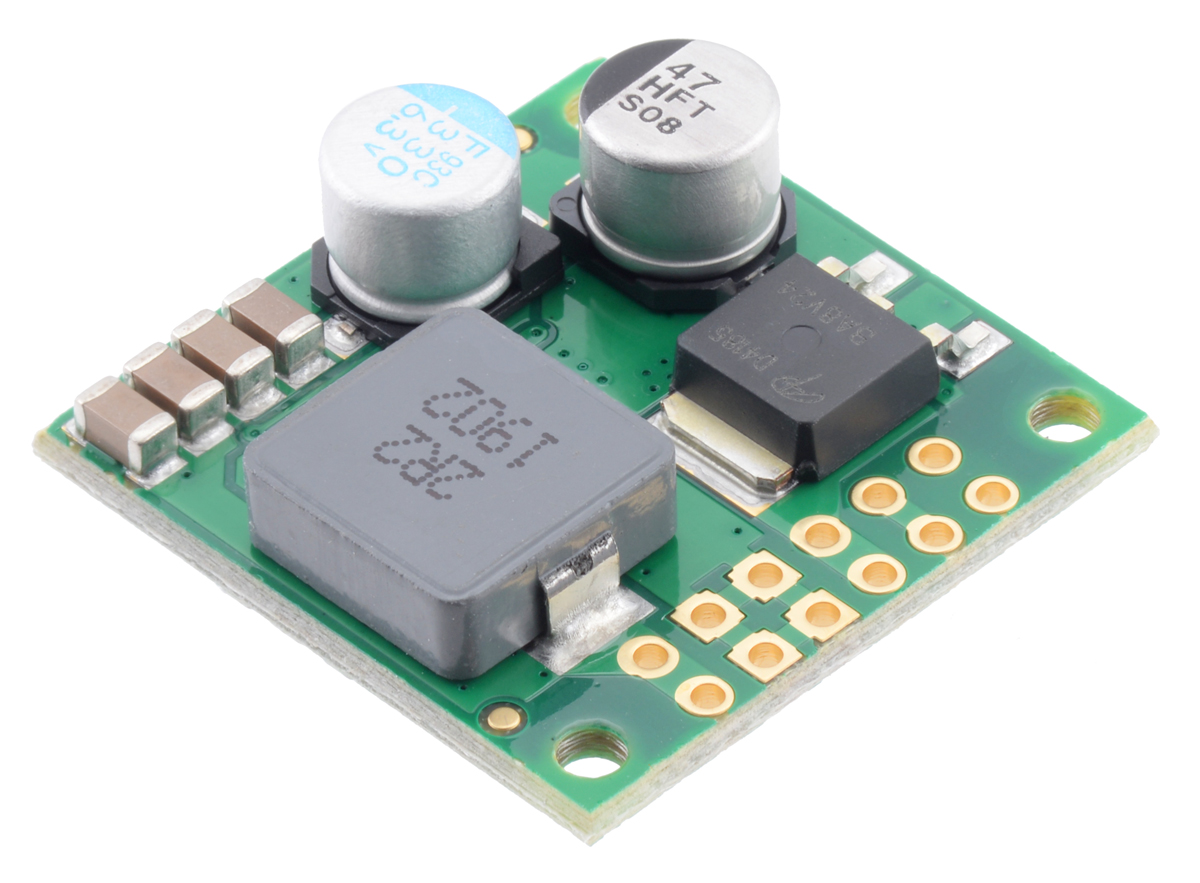
\includegraphics[width=0.5\textwidth]{img/polulu5V8A.jpg}
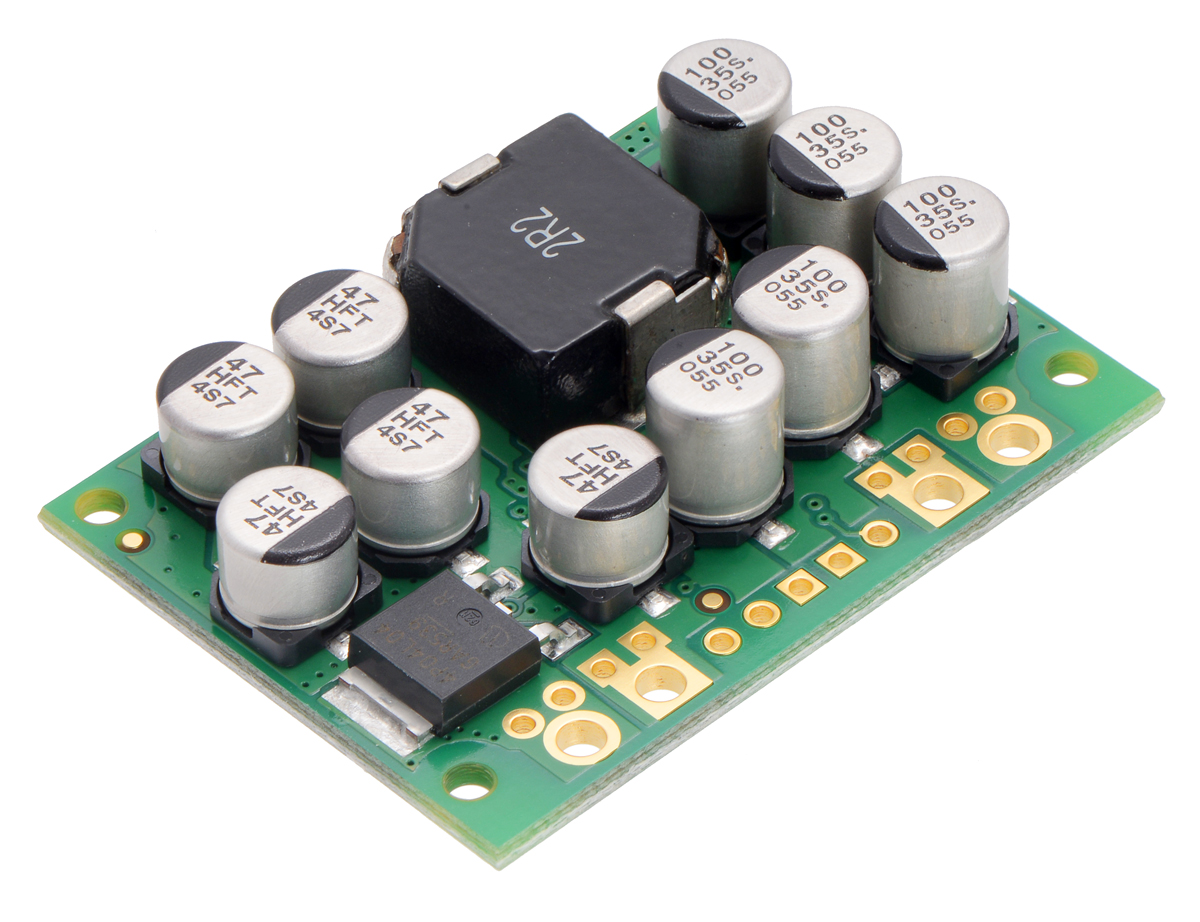
\includegraphics[width=0.5\textwidth]{img/polulu6V15A.jpg}
\caption{Zakupione przetwornice \cite{polulu_step_down}}
\label{img:voltage_converters}
\end{figure}

%https://botland.com.pl/serwa-typu-standard/9182-serwo-feetech-ft5715m-standard-5904422312756.html
%https://botland.com.pl/serwa-typu-standard/3576-serwo-powerhd-lf-20mg-standard-6939670200387.html